\chapter{Memory Controller Architecture}
\label{chap:arch}
\section{Memory Hierarchy Organization}
\begin{figure}
    \centering
    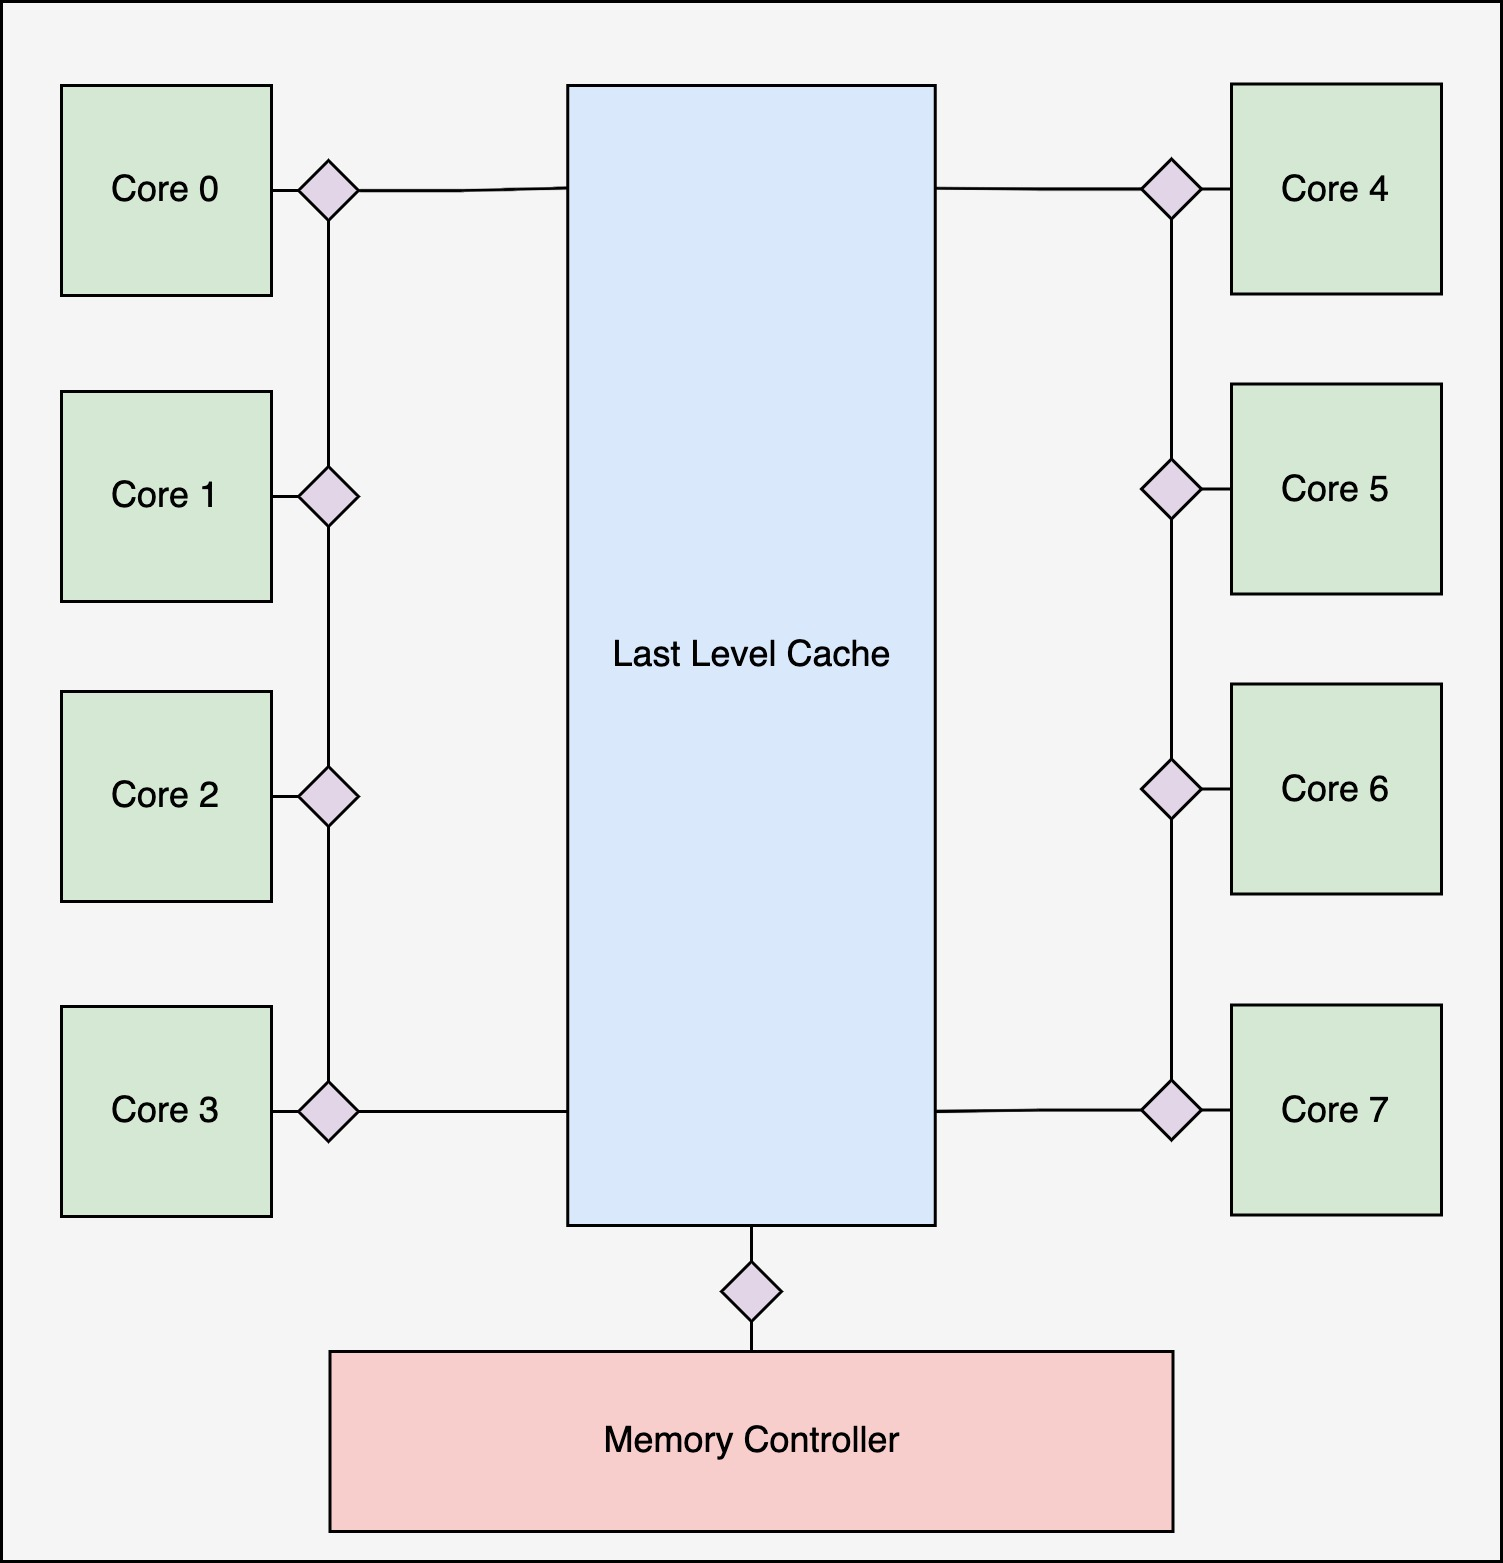
\includegraphics[scale=0.15]{images/soc-2.jpg}
    \caption{A modern SoC with 8 cores and last-level cache.}
    \label{fig:soc-2}
\end{figure}
An SoC design is organized as nodes of processing elements such as CPUs or accelerators, on-die memory systems such as L2 caches or Last Level Cache (LLC), and memory and IO controllers. A DRAM controller in such systems provides backing memory to the whole system and allows for larger programs and data to be processed on the die by caching the working subset of memory. Figure \ref{fig:soc} shows a modern memory hierarchy and system. CPU clusters are shown to have private level one and two caches; a system-level cache provides a larger pool of memory and is backed by DRAM. This project pieces together the memory controller and the physical layer to be used for the future implementation of such systems. In Figure \ref{fig:soc-2} and \ref{fig:soc}, a modern SoC is depicted with eight processing elements, a shared LLC, and a memory controller. The purple diamonds are routers as part of the SoC interconnects. One such node is connected to the memory controller. 

\begin{figure}[b]
  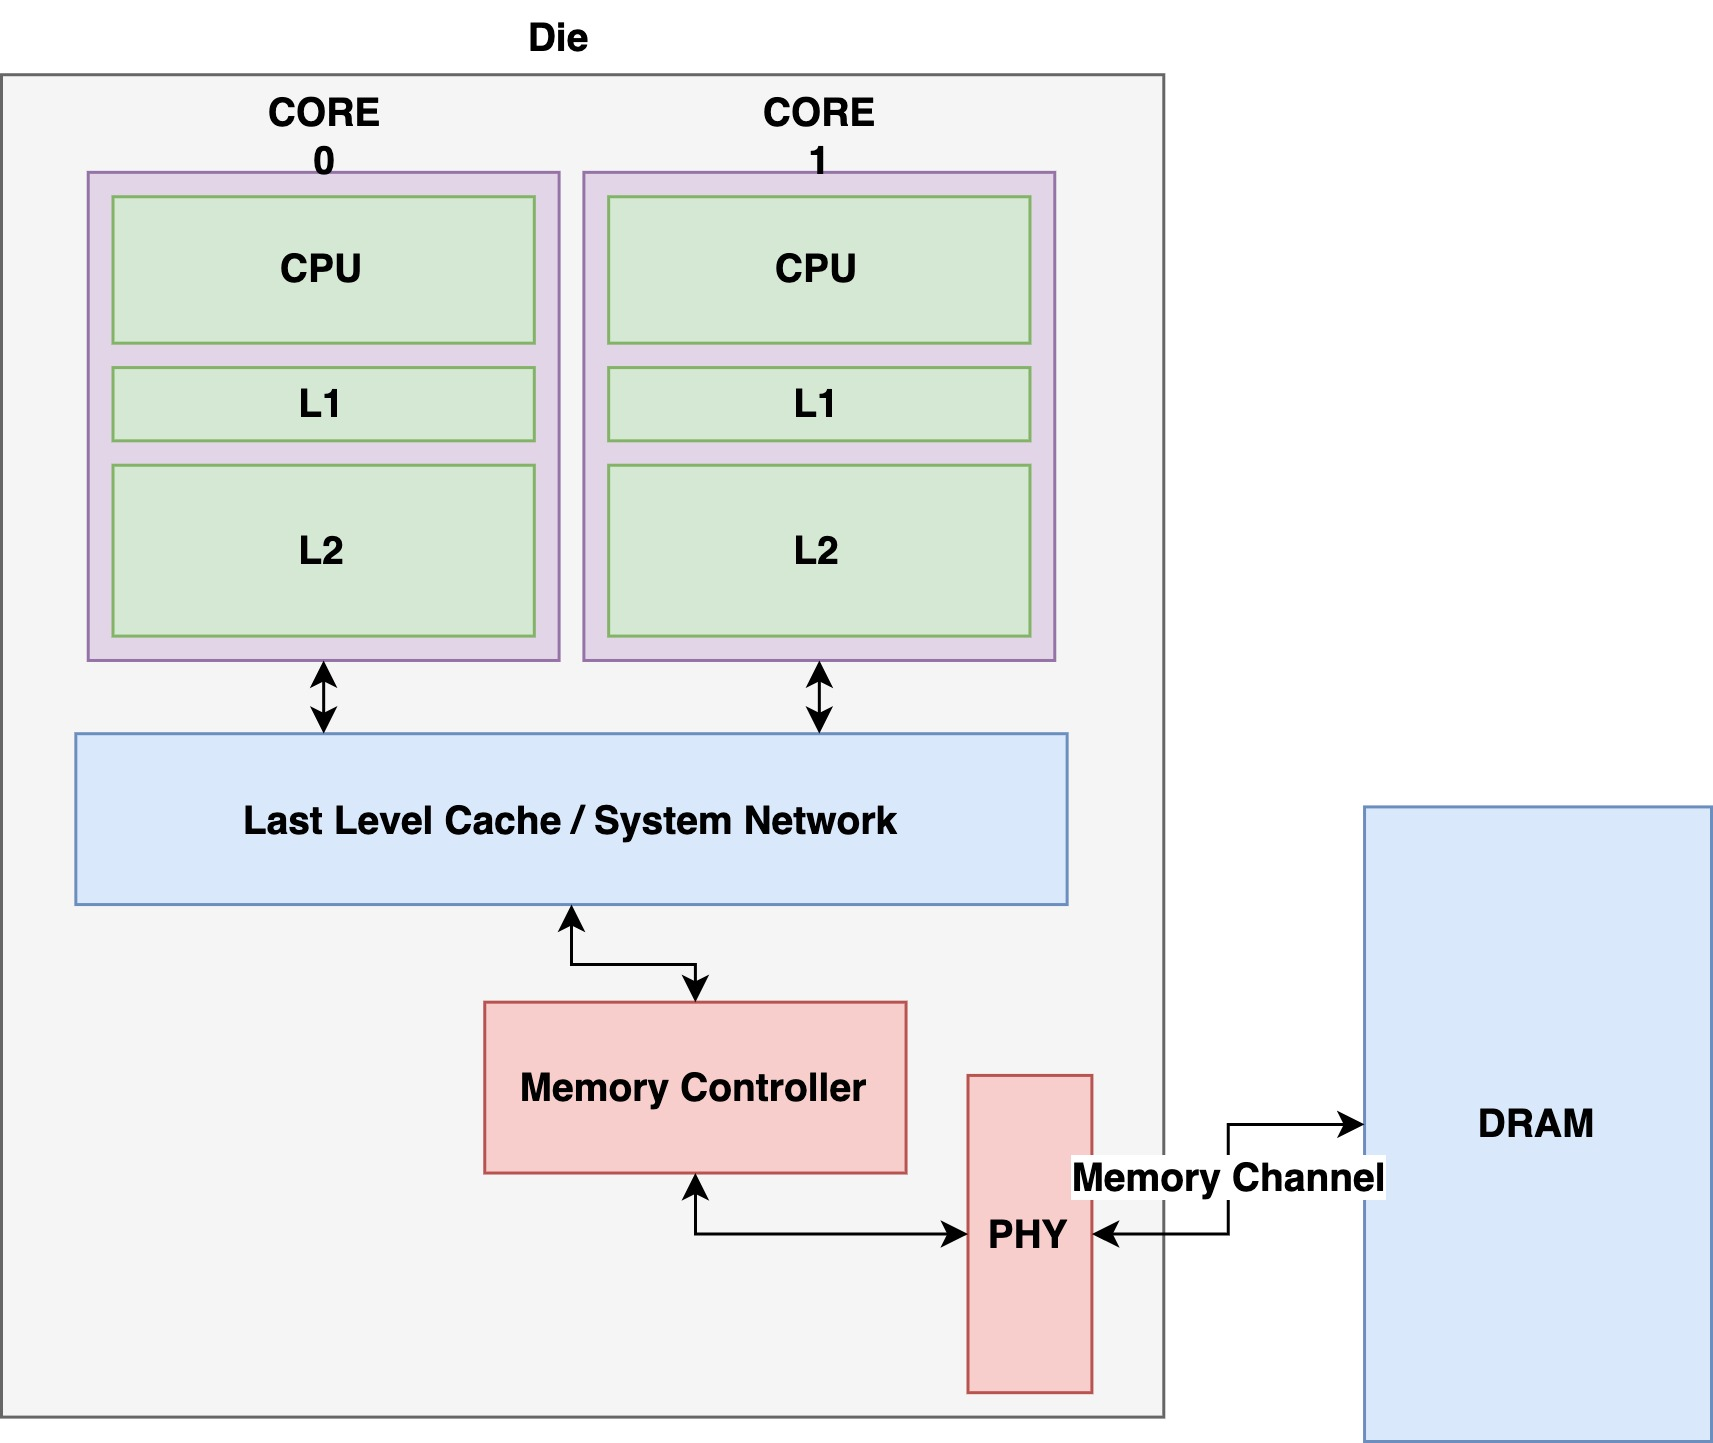
\includegraphics[scale=.15]{images/soc.jpg}
  \caption{Logical view of the memory hierarchy.}
  \label{fig:soc}
\end{figure}


As SoC architects, we should be able to perform early-stage modeling of systems by taking advantage of software modeling. A DRAM controller software model gives early estimates of system-level performance and bottlenecks. Rapid cycles of RTL software modeling is the approach taken to design complex systems. This implementation of the LPDDR4 memory controller allows for such models to be deployed and connected to the LPDDR4 model as well for more realistic performance analysis.
\section{TileLink Front-end}


\begin{figure}
    \centering
    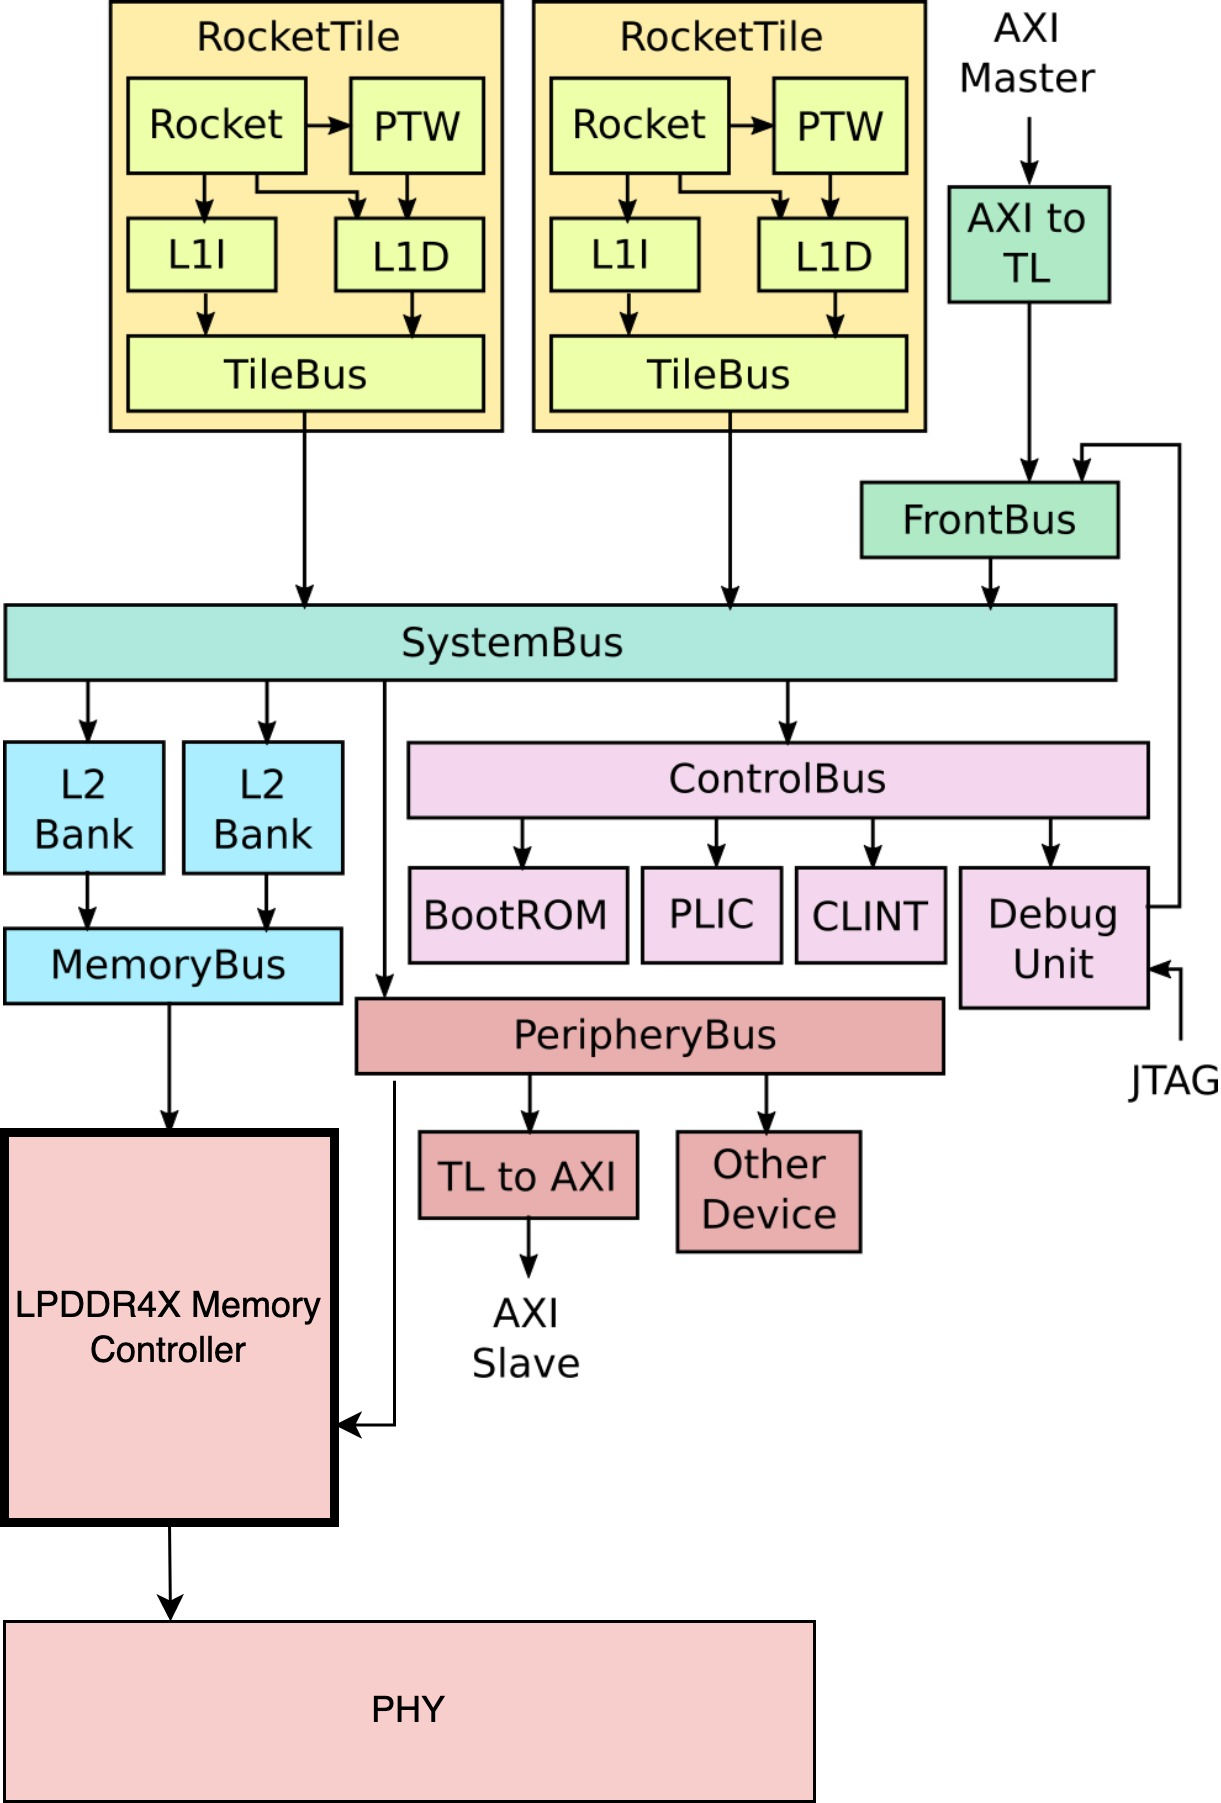
\includegraphics[scale=0.2]{images/bus.jpg}
    \caption{Bus hierarchy with LPDDR4X controller.}
    \label{fig:bus}
\end{figure}

TileLink is a logical transmission protocol to communicate messages, data, and cache coherency packets to other agents in the system \cite{tilelink}. During the design elaboration, TileLink agents of the system perform an agreement to ensure that the system is connected logically, and is free of problems such as deadlocks. For that, Chipyard \cite{chipyard}, an SoC generator, uses diplomacy to conduct the diplomatic agreement between all the agents in the system. This agreement happens at compilation time such that the system is guaranteed to have no cycles. The Diplomacy directed acyclic graph or DAG generates an SoC configuration to be elaborated. TileLink differentiates the nodes in the system based on which node is a source and which node is a sink node. A manager node (sink node) is a node that takes in requests and provides responses. TileLink protocol requires the implementation of channels A and D for a manager agent. On the other hand, a client node is a node that issues requests to other agents in the system. A CPU core in the system has a client node attached to its interface to the network. On the other hand, the memory controller has a manager node to receive requests and respond to them. To implement an interface for an SoC, the DDR controller instantiates a manager node and connects it to the memory bus of the system. In the context of the memory controller, the manager node receives only put and get requests over channel A. A put request is a data transfer from a client node to the manager node such as a write-back to a lower-level cache. Similarly, a get request is a request for data from an address. The manager node is able to respond to the requests over channel D. In addition to the manager node, the DDR controller requires a register node for the configuration of the internal registers. Figure \ref{fig:bus} shows the bus hierarchy in Chipyard and the connection of the LPDDR4X controller to the memory bus and periphery bus. Figure \ref{fig:reg-node} shows the register node is connected to the periphery bus or the PBUS of the system. The register node is needed for providing the controller with a register space that software can write to. The registers are used to control the timing parameters described in the next chapter, control and status registers, and mode registers of the DRAM device.  Each manager node can use the A and D channels of TileLink. Requests are delivered to the manager node via the A channel, and responses are delivered to the network via the D channel. Figure \ref{fig:tli}  shows a block diagram of the manager node in more detail. The logic within the manager node needs to provide two decoupled (ready-valid) interfaces to each side of the module.

\begin{figure}
    \centering
    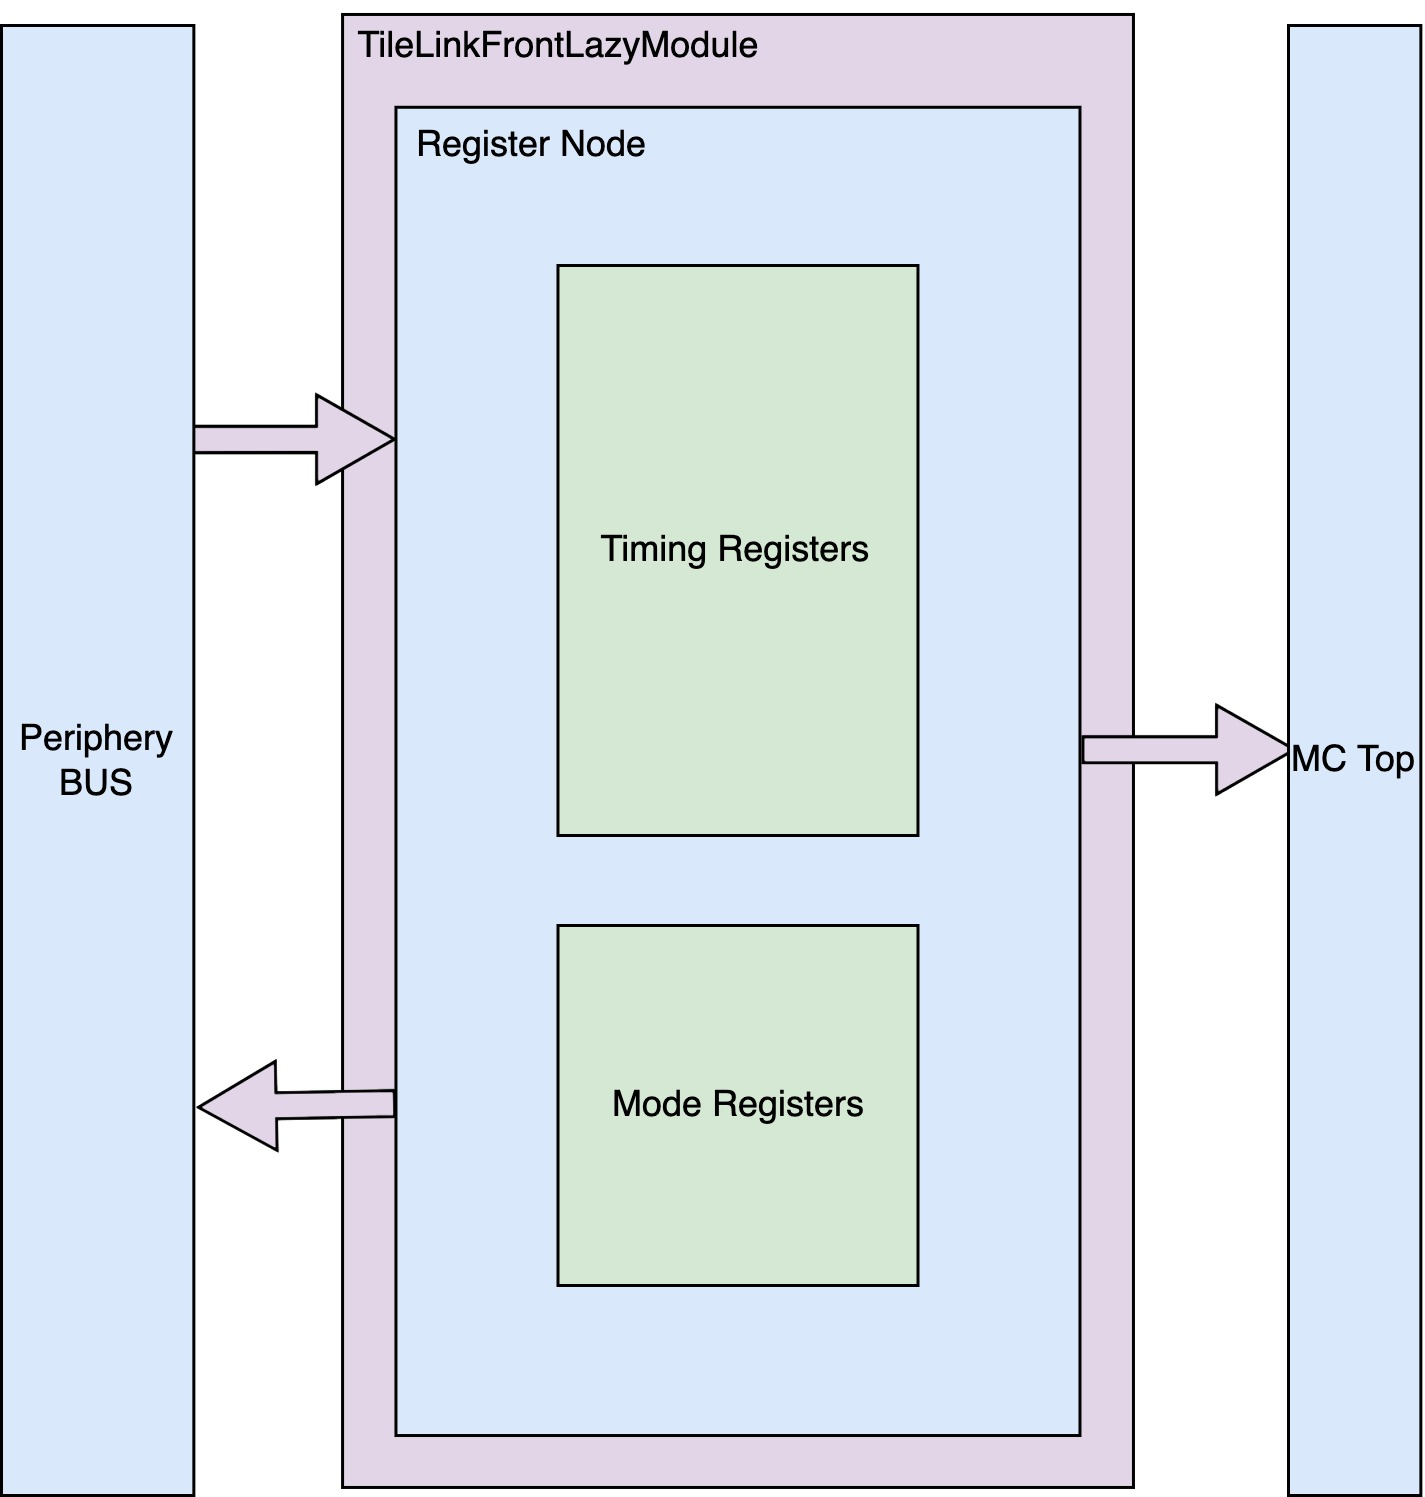
\includegraphics[scale=0.1]{images/reg-node.jpg}
    \caption{Register node.}
    \label{fig:reg-node}
\end{figure}
\begin{figure}
    \centering
    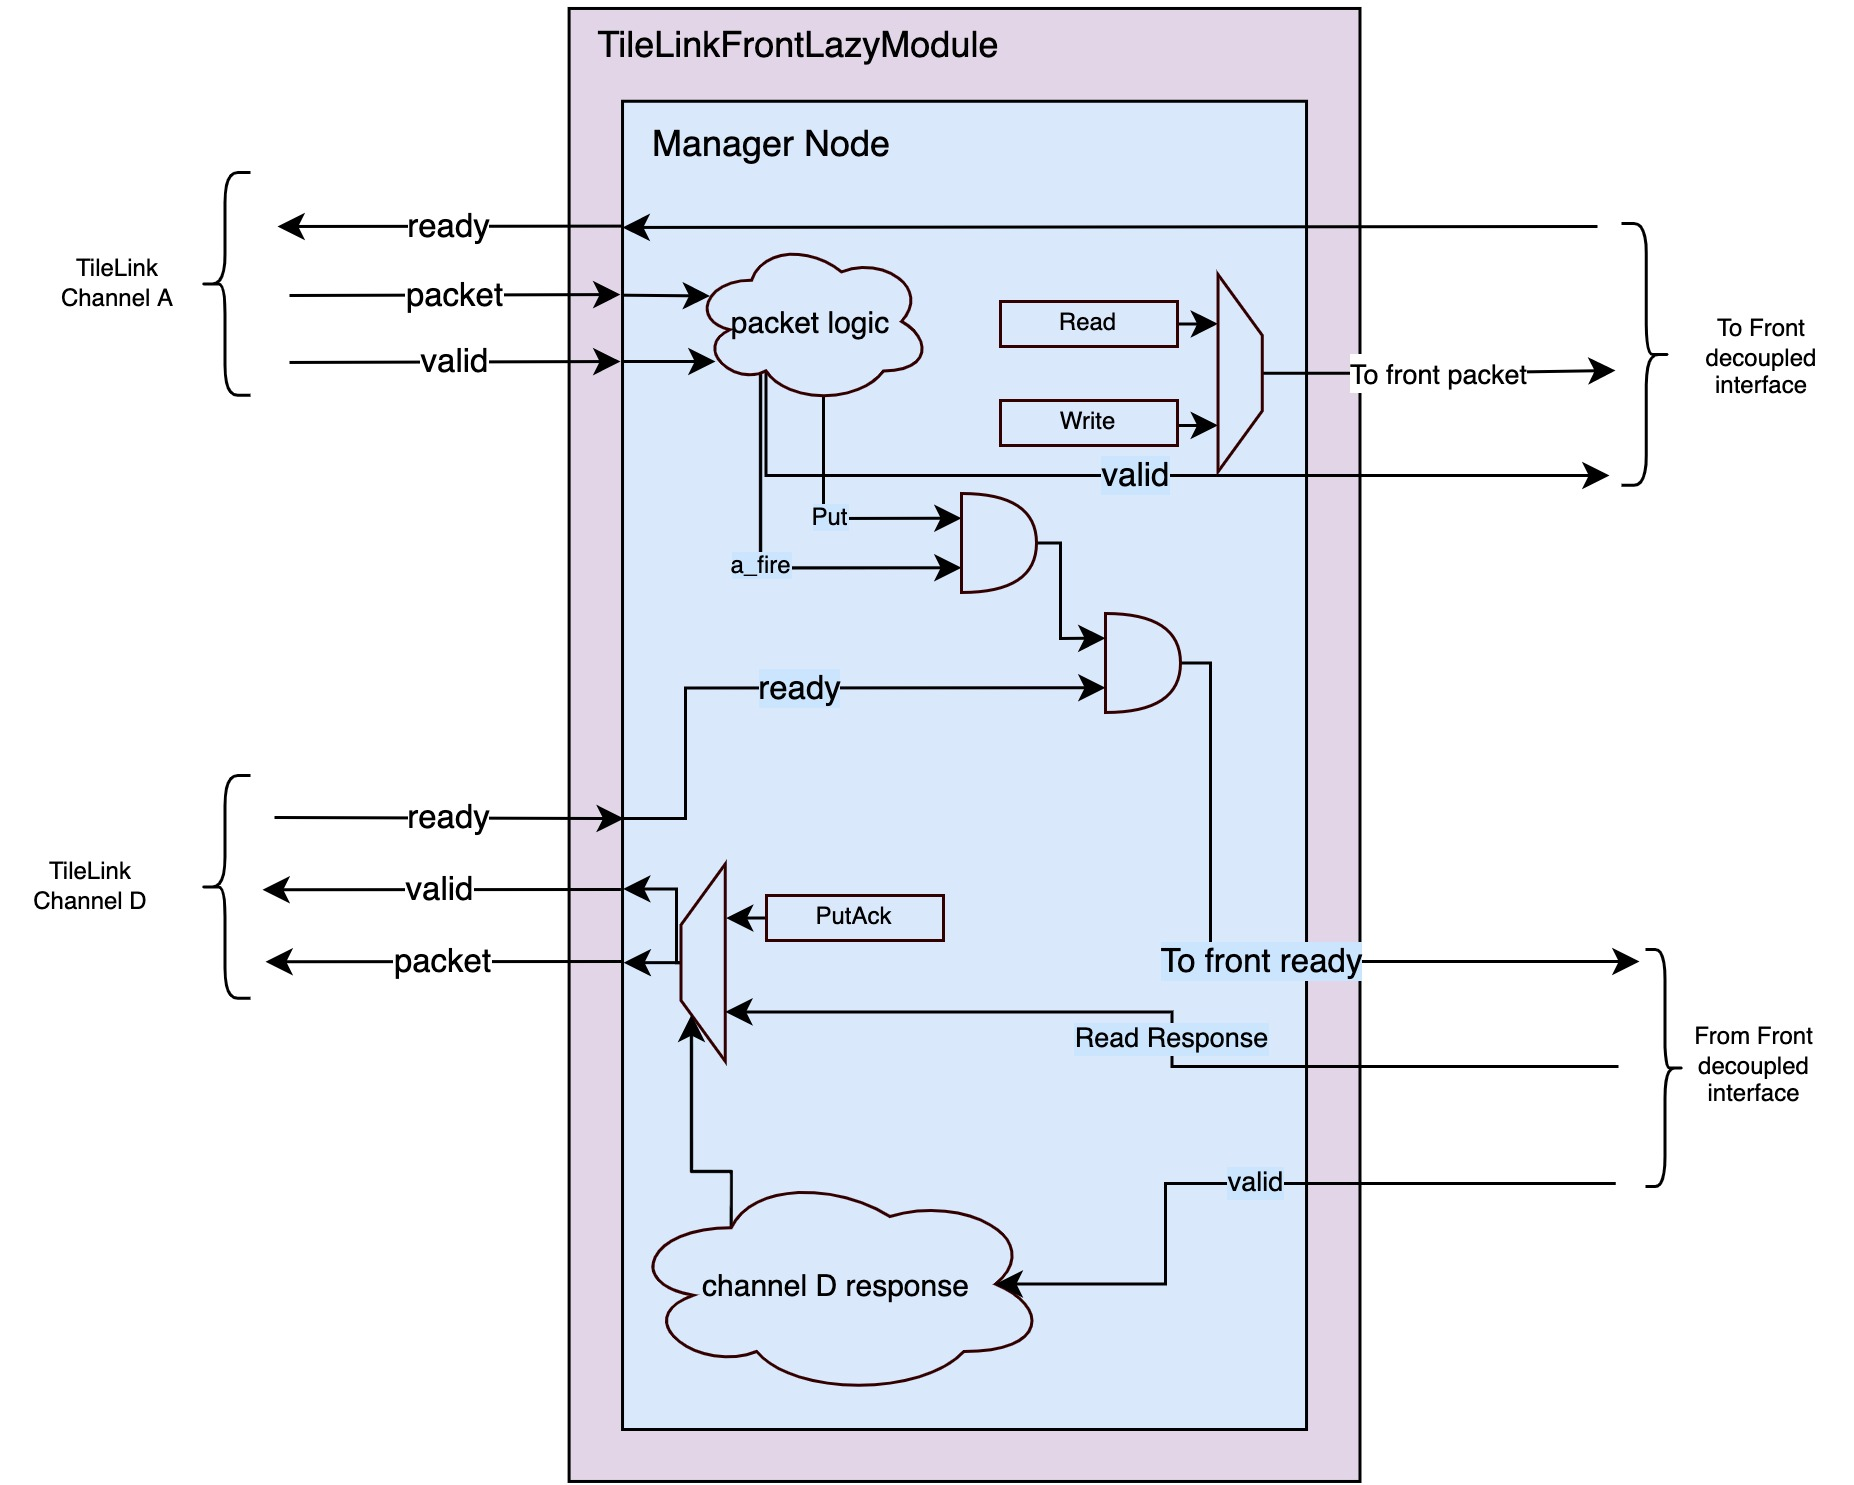
\includegraphics[scale=0.18]{images/tl-front.jpg}
    \caption{TileLink interface.}
    \label{fig:tli}
\end{figure}

A code snippet that instantiates the manager node with the parameters provided to the DDDR configuration case class is shown below. Some of the important parameters are the base address, region type, and beat byte. The beat bytes variable indicates the data width for each cycle of the transfer. Region Type of uncached indicates that the data has not been yet cached and the agent that requested this data needs to cache it. 
\begin{verbatim}
val device = new SimpleDevice("ddr-front", Seq("ddr,ddr0"))
val beatBytes = tlParams.BEATSIZE / 8
val node = TLManagerNode(Seq(TLSlavePortParameters.v1(
    Seq(TLSlaveParameters.v1(
      address = Seq(AddressSet(tlParams.ADDRESS, tlParams.SIZE)),
      resources = device.reg,
      regionType = RegionType.UNCACHED,
      executable = true,
      supportsGet = TransferSizes(1, beatBytes),
      supportsPutFull = TransferSizes(1, beatBytes),
      supportsPutPartial = TransferSizes(1, beatBytes),
      fifoId = Some(0))),
    beatBytes = beatBytes)))
\end{verbatim}

The TileLink module captures the requests arriving through the A channel. These requests are then determined to be either a write or read request based on the packet header and opcode bits. Every write request is responded to with an acknowledgment on the D channel immediately. The acknowledgment of the put requests establishes that the put request has been registered by this agent. The read requests are responded to after the data is read from the device and is ready to be sent to the requesting agent in the system. The logic in the TileLink module needs to translate the TileLink standard packets to an internal protocol bundle as shown below. 
\begin{verbatim}
class FrontToDP extends Bundle {
  val isWrite       = Output(Bool())
  val data          = Output(UInt((geom.TOTALBITS).W))
  val address       = Output(UInt((geom.FULLADDRBITS).W))
  val byteEnable    = Output(UInt((geom.TLBYTEEN).W))
  val requesterID   = Output(UInt((tlParams.RIDW).W))
  val bankNo        = Output(UInt(3.W))
}
\end{verbatim}
Once the responses to the read commands are ready, the memory controller datapath transfers the data to the TileLink module using the bundle shown below. 
\begin{verbatim}
    
class DataPacket extends Bundle {
  val hw            = Output(Vec(geom.TOTALBITS/dfi.DWIDTH, UInt(dfi.DWIDTH.W)))
  val requesterID   = Output(UInt((tlParams.MASTERIDSIZE).W))
}
\end{verbatim}
The hw field in the DataPacket corresponds to half-word data fields. A total of 256 bits of data is retrieved from the memory and is concatenated together as half-word data fields in this packet. The memory controller front-end logic guarantees an in-order response to the read requests. This needs to be handled by the datapath since the memory controller core might issue the requests to separate banks out-of-order. Every read transaction that is ready to be sent out to the SoC must go through the TileLink module logic. The internal packets are then translated to TileLink AccessAckData responses.
\section{Asynchronous Crossing}
The memory controller must adhere to a specific speed bin determined by the JEDEC specification. This frequency determines the frequency of the memory controller and the PHY. In this project, we targeted a frequency ratio of 1:4 between the memory controller and the PHY. This frequency ratio gives rise to 1:4 mapping commands from the memory controller to the clock phases of the PHY. In addition, the SoC might be running at a much higher frequency than the memory controller. To perform a clock domain crossing we have placed an asynchronous FIFO in between the TileLink module and the datapath of our design. The block diagram in Figure \ref{fig:cdc} shows the crossing point between the SoC domain and the controller domain. 

To determine the queue size for the asynchronous FIFO, a sampling frequency on the consumer side, and a producing frequency is needed. Given a frequency ratio of 2 to 1 from SoC to MC and assuming the worst-case scenario of en-queuing transactions with MC not ready:\\
    \indent SoC frequency = 800 MHz \\
    \indent MC frequency = 200 MHz \\
    \indent Burst Length = $b$ requests\\
    \indent Maximum enqueue frequency = $1 \frac{request}{cycle} * \frac{800 cycles}{1 s} = 800 \frac{requests}{s}$\\
    \indent Total time to write $b$ requests = $\frac{b}{800} s$\\
    \indent Maximum dequeue rate = $1 \frac{request}{cycle} * 200 \frac{cycles}{s} = 200 \frac{requests}{s}$\\
    \indent Maximum number of dequeues during the burst = $\frac{b}{800} s * 200 \frac{requests}{s} = \frac{b}{4} requests$\\
    \indent Number of transactions to be stored in the queue = $b - \frac{b}{4} = \frac{3b}{4}$\\
    
With the burst length of $b$ and 800 MHz frequency to a 200 MHz frequency, we would need to have a buffer depth of $\frac{b}{4}$. In addition, a designer needs to perform workloads and simulate the design at the system level to understand the depth necessary such that the FIFO would not become the bottleneck of the system.

\begin{figure}[h]
    \centering
    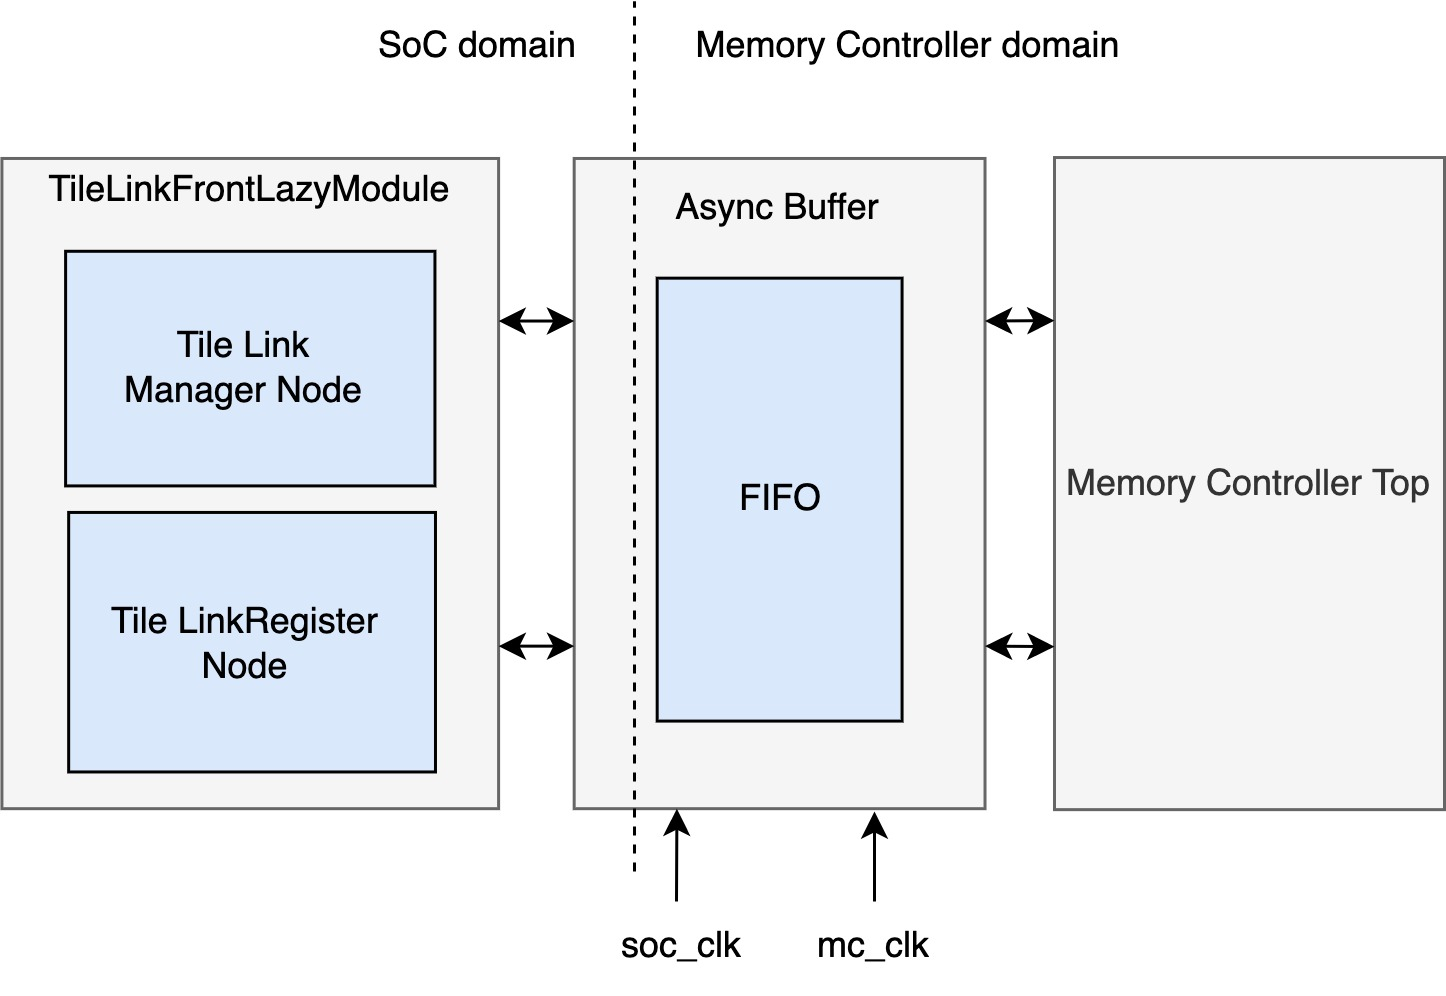
\includegraphics[scale=0.2]{images/cdc.jpg}
    \caption{Asynchronous crossing.}
    \label{fig:cdc}
\end{figure}
\newpage
\section{Controller Datapath}
The memory controller datapath takes in read and writes packets that are passed by the TileLink module. These packets have an internal format and are processed in the controller datapath. \footnote{The architecture planning and design of this unit in the design were done by Ken and me. The implementation of the sub-modules was a shared effort by Ken Ho and me.} 

The memory controller datapath contains ID assignment logic and dispatching logic to bank machines. In addition, the datapath has ports to insert data into the internal read and write queues. The datapath covers the read and writes queues units; the datapath is connected to two different points of the design, the front-end TileLink module, and the DFI module. DFI is a protocol specification to bridge between the controller and the PHY \cite{dfi}. The datapath is also responsible for changing the addressing scheme to DRAM-specific addressing. TileLink addresses must then be sliced into the bank address, row address, and column address which are all defined by the DDR device capacity and organization. The bank address must be from 0 to 7 and requires 3 bits of the address. In order to interleave the requests among different banks, we dedicated 3 bits of the address between the column and row addresses. Row address spans a larger number of bits of the address and is also dependent on the target DDR device and capacity. Column address takes up the lower bits of the address to slice into the rows and select a subset of bits from the row buffer. A breakdown of the physical addresses is shown in Figure \ref{fig:addr}.
\begin{figure}
    \centering
    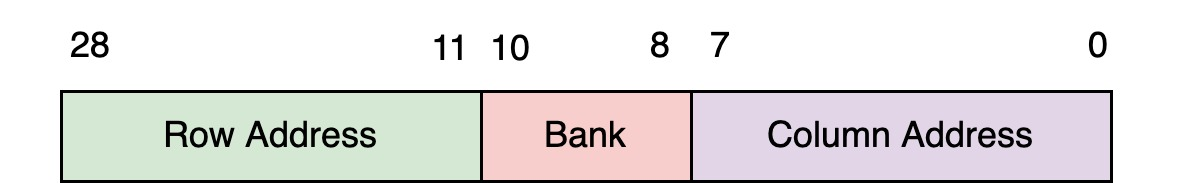
\includegraphics[scale=0.3]{images/address.jpg}
    \caption{Breakdown of physical address.}
    \label{fig:addr}
\end{figure}

Assignment of an ID to each transaction as they enter the controller is required for further referencing the transaction. As an example, a PUT transaction is entered into the datapath and is given a transaction ID. Furthermore, it enters the write queue where the data and transaction IDs are stored in an SRAM. Once the core logic processes the transaction and timing parameters are checked, the request can cross the controller and PHY interface. At this stage, the write data needs to be sent out to the PHY as well as the control signals. The transaction is identified using the previously assigned ID and is retrieved from the SRAM to be sent to PHY. A similar procedure applies to a read transaction that enters the controller. Once a read transaction enters the datapath, an ID is assigned to the transactions. A bundle with the necessary metadata is then stored in the read queue for further processing of the read transaction. Once the read transaction is processed and the data is retrieved from the device, the read queue is referenced, and both the data and transaction metadata are stored in the read SRAMs. The ID can also be used to identify the relative age of a pending transaction in the queues as the ID generation is an incremental counter. 

The bank machines internal queues and the main transaction queue control the ready signal outputted from the datapath. The ready signal is then translated and connected to the asynchronous FIFO which in turn exposes another ready signal to the TileLink module. Once the ready signal is low, the senders in the SoC would need to re-try sending their packets. The TileLink module in the design takes the responsibility of receiving TileLink messages over channel A and sending them back over Channel D as mentioned in section 2.2.
\subsection{Transaction Queue}
A main transaction queue is used to store the requests as they enter the datapath. The queue is also used to provide a ready signal to the asynchronous FIFO and the TileLink module. The metadata and the transaction itself are stored in the queue. The transaction fields and metadata are write enable (we), address (addr), ID (cmdID), mask (byteEnable), bank (bankNo), and requester ID shown below:
\begin{verbatim}
class BankInPacket (val geom : GeomParams) extends Bundle {
  val we            = Output(Bool()) // write enable
  val addr          = Output(UInt((geom.FULLADDRBITS).W))
  val cmdID         = Output(UInt((geom.IDBITS).W))
  val byteEnable    = Output(UInt((geom.TLBYTEEN).W))
  val bankNo        = Output(UInt(3.W))
  val requesterID   = Output(UInt(tlParams.MASTERIDSIZE.W))
}
\end{verbatim}
\subsection{Read Queue}
The read queue module contains the read queue with the corresponding SRAMs and a read in-order queue for enforcing the ordering of read responses. 

The purpose of having a read-in-order queue is to guarantee the same ordering of read responses to the system as the memory controller received. A usual optimization is to avoid such guarantees; however, having this scheme allows us to keep track of transaction processing times, and quality of service at a system or NoC level. 

The read transactions enter the read-in-order queue as they enter the read queue module. Similarly, the data that was previously requested by the controller to the DRAM device can be inserted into the read SRAMS at any cycle that the data is received by the controller. Once the SRAM row is filled with the requested data, the row is set to be filled using a per-row bit vector. On every cycle, if there exists a pending read transaction in the read-in-order queue and the data corresponding to that transaction is available in the read SRAMs, the transaction at the top of the queue is dequeued. The dequeued read transaction is the oldest pending transaction with ready data available in the read SRAMS.

The read queue contains eight SRAM banks in parallel providing a total of 256 bits wide data. The depth of the SRAMs is parameterized by the designer; however, the depth of the SRAMs determines whether or not the controller can issue a read command. A one-bit valid signal per row is used to indicate if the row is empty or allocated. An allocate request is issued to the module by the datapath once the read transaction is entered into the datapath. The read transaction allocates a row in the SRAM and enqueues the transaction into the read in-order queue. Once the data is received by the DFI module, the 256-bit wide data is entered into the previously allocated SRAM row. The address of the SRAM row is determined using a Content Addressable Memory table (CAM table). The data is then stored in the allocated SRAM row using the address found from the CAM. Transaction IDs are used to compare and find the addresses from the CAM table. A block diagram of the read queue is depicted in Figure \ref{fig:reqdq}. 

The designer of the SoC should configure the depth of the queues appropriately and pay attention to the maximum allowable pending transaction. It is very important to note that a read transaction that is serviced and responded to by the DRAM device enters the controller and is captured by the logic in the read queue and the SRAMs. As a result, if a read transaction that is at the head of the read-in-order queue enters the pipeline, it will not be sent to the SoC immediately as a read and write to an SRAMs row must not occur on the same cycle.

In the case of lower-depth queues, a designer may choose to avoid SRAMs and map the memory logic to register-based memory banks.
\begin{figure}[H]
    \centering
    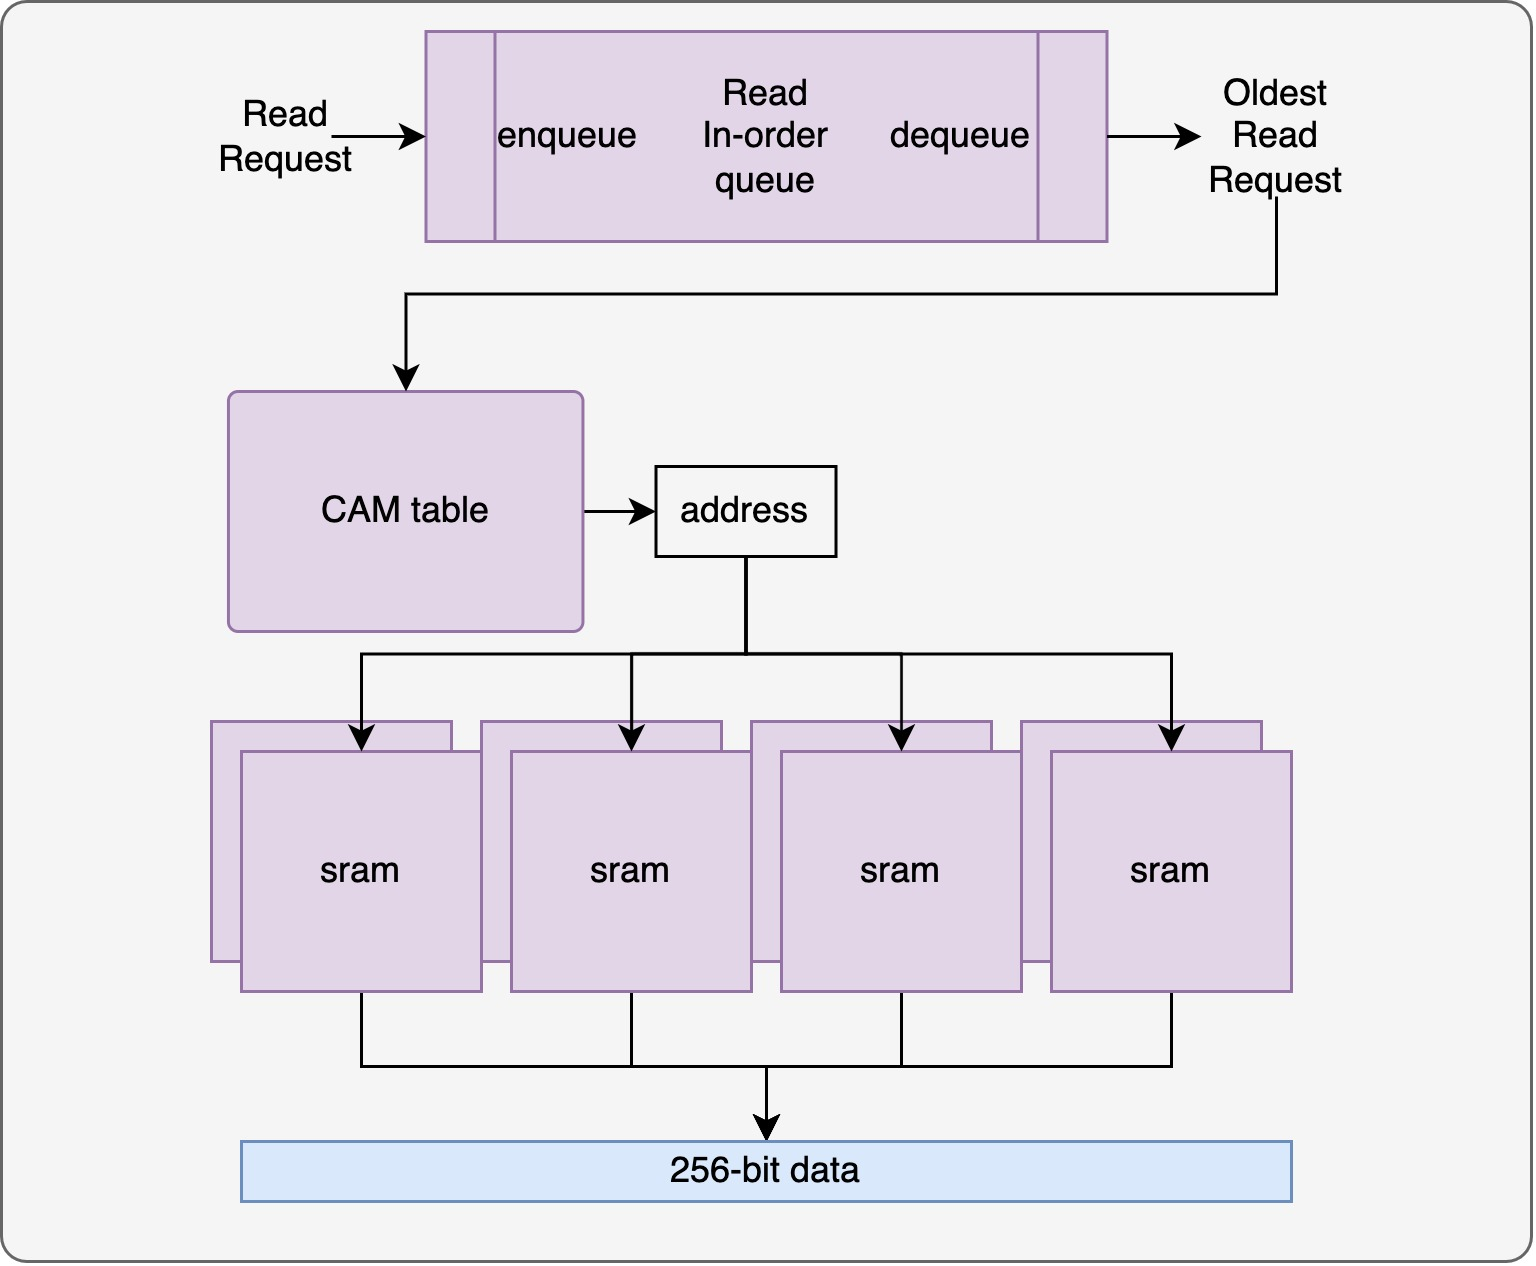
\includegraphics[scale=0.2]{images/readQ.jpg}
    \caption{Read queue.}
    \label{fig:reqdq}
\end{figure}
\subsection{Write Queue}
Similar to the read queue, a module is dedicated to keeping the write transactions within the datapath until the write transaction is processed and ready to be issued to the PHY interface. 
The write queue contains eight SRAMs to store a total of 256 bits of data internally. Every write transaction enters the write queue; the data corresponding to the write with the ID of the transaction is stored in an empty row of the write SRAMs. The address of the SRAM row is stored in a CAM table that is accessed in the future using the transaction ID. A high-level block diagram of the write queue is shown in Figure \ref{fig:wrQ}.
\begin{figure}
    \centering
    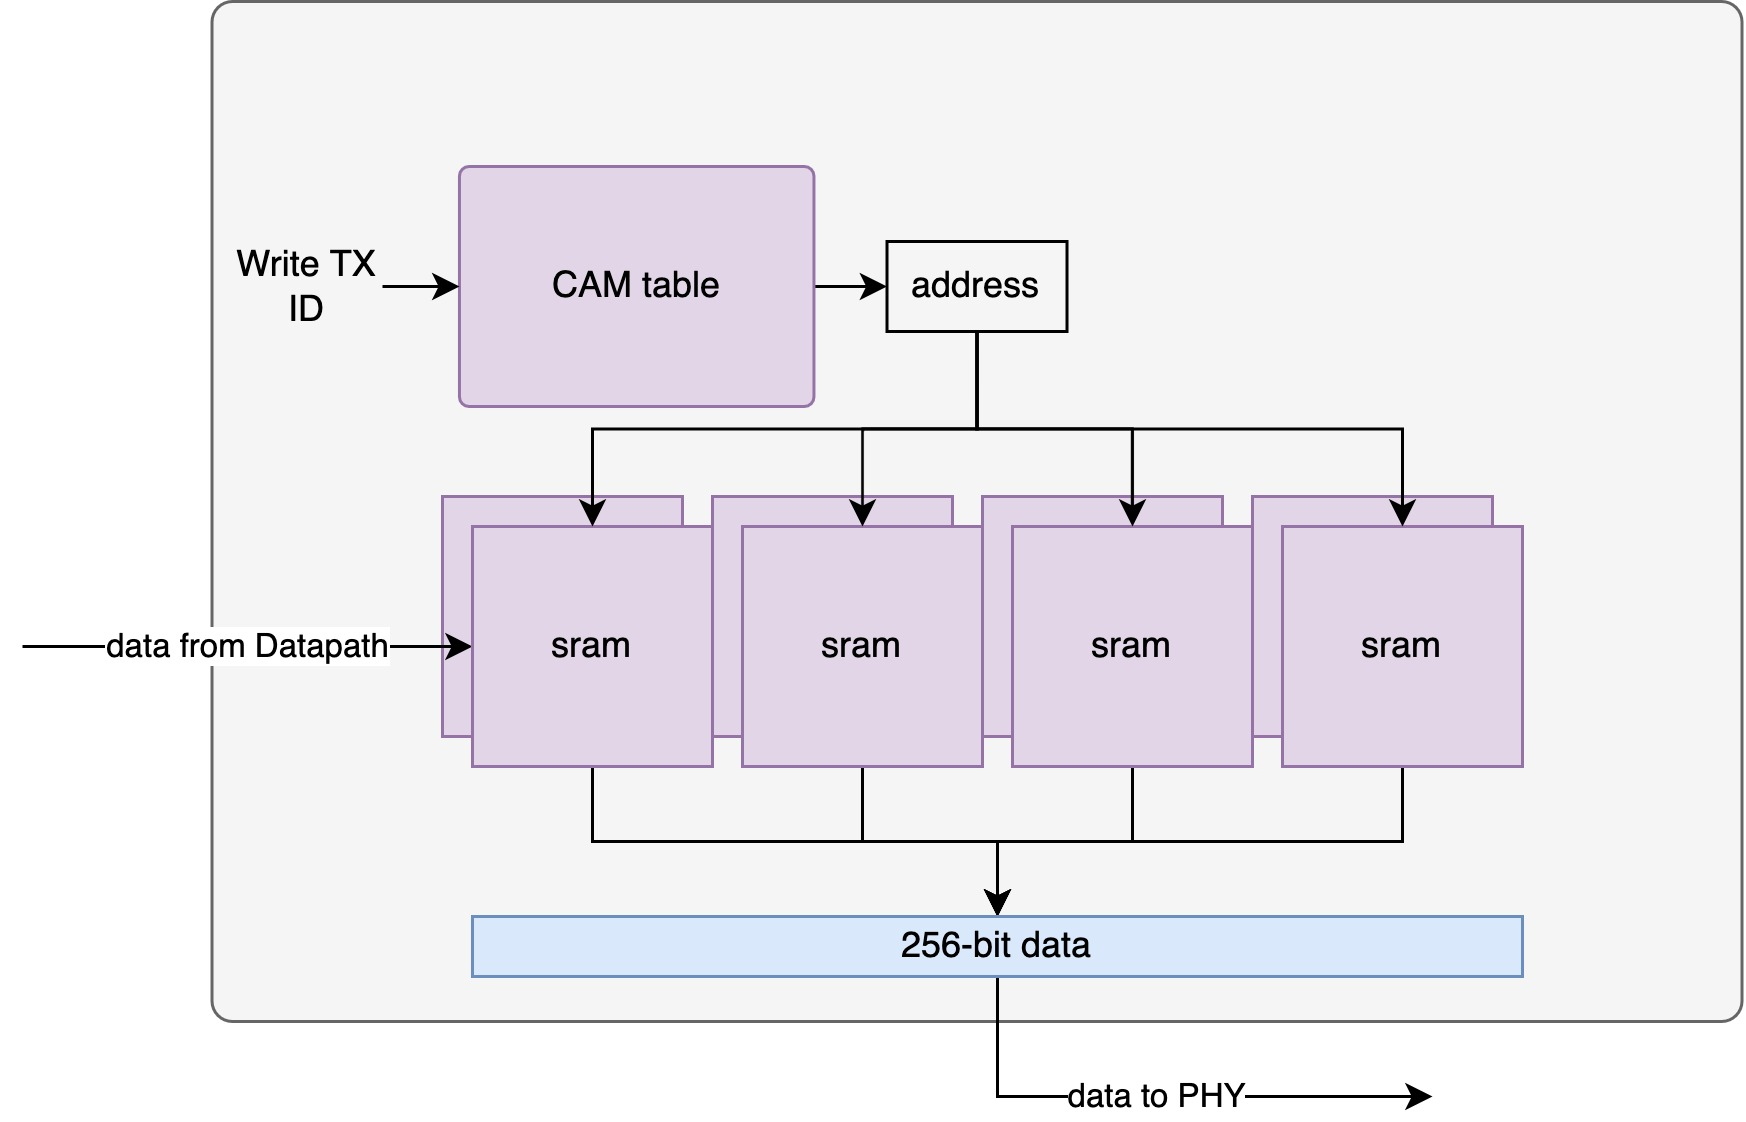
\includegraphics[scale=0.2]{images/wrQ.jpg}
    \caption{Write queue.}
    \label{fig:wrQ}
\end{figure}
\section{Bank Machines}
The controller core contains eight Bank Machine modules each of which keeps track of the state of a bank in one rank of the DRAM device. A diagram of the FSM that each bank machine implements is shown in Figure \ref{fig:fsm}. \footnote{The architecture planning of this unit was a shared effort by Ken Ho and me. Implementation of this unit referenced LiteDRAM implementation \cite{enjoydigital}. Verification of the unit was done by Ken Ho.
}

A bank machine implements the JEDEC state machine for each bank with the additional functionality of ensuring the timing parameters are met. 
A memory transaction is split into at least two commands each of which has its own timing parameters. Table \ref{tab:cmd} shows a summary of the commands that the memory controller needs to issue. A read transaction to an address that was not read by the controller recently must issue a row activate command to the device first. The row activate command (RAS) is issued to the device so that the word line corresponding to the address is activated and the content of the row is sensed and registered into the row buffer. A read or a write command is considered a column access command (CAS). This command requires us to wait for TRCD parameter, which is some number of cycles specified by JEDEC specification. Another important timing parameter is TCCD which denotes the delay between two consecutive column access commands. For the read transaction to be safely issued to the device, all the relevant parameters must be checked beforehand. A legal command then can be issued to the device. 

A timing controller in the design refers to a counter that is restarted with the same value for each timing parameter. The timing parameters can be set using the TileLink register node. A core can be used to write data into a specific register that is mapped to a timing parameter. In an ASIC design, this gives the designer flexibility to modify a timing parameter at the time of the chip bring-up. In Figure \ref{fig:fsm}, a simplified version of the JEDEC state machine is shown. The bank machines have internal counter controllers for each timing parameter in addition to implementing this FSM.

The ordering of each command is specified by this FSM. However, there are additional queues in the bank machines in order to compare multiple transaction addresses to keep a row active in case of a hit. This optimization can be further used to re-order transactions in the queues such that we can perform multiple CAS commands on the same activated row. This reduces the overhead of RAS commands. 
\begin{table}
    \centering
    \begin{tabular}{c|c}
        Command & Description \\
        \hline
        Activate & Row access, Activates a row\\
        Read & Column access, reads a subset of the row\\
        Write & Column access, writes to a subset of the row\\
        Precharge & Precharges the row to an idle state\\
        Auto-precharge & Automatic precharge after a read or write\\
        Refresh & Refreshes the bank to preserve the data\\
        Refresh all & Refreshes all the banks\\
        Precharge all & Precharges all the banks, all go to idle state
    \end{tabular}
    \caption{LPDDR4X standard commands.}
    \label{tab:cmd}
\end{table}

\begin{figure}
    \centering
    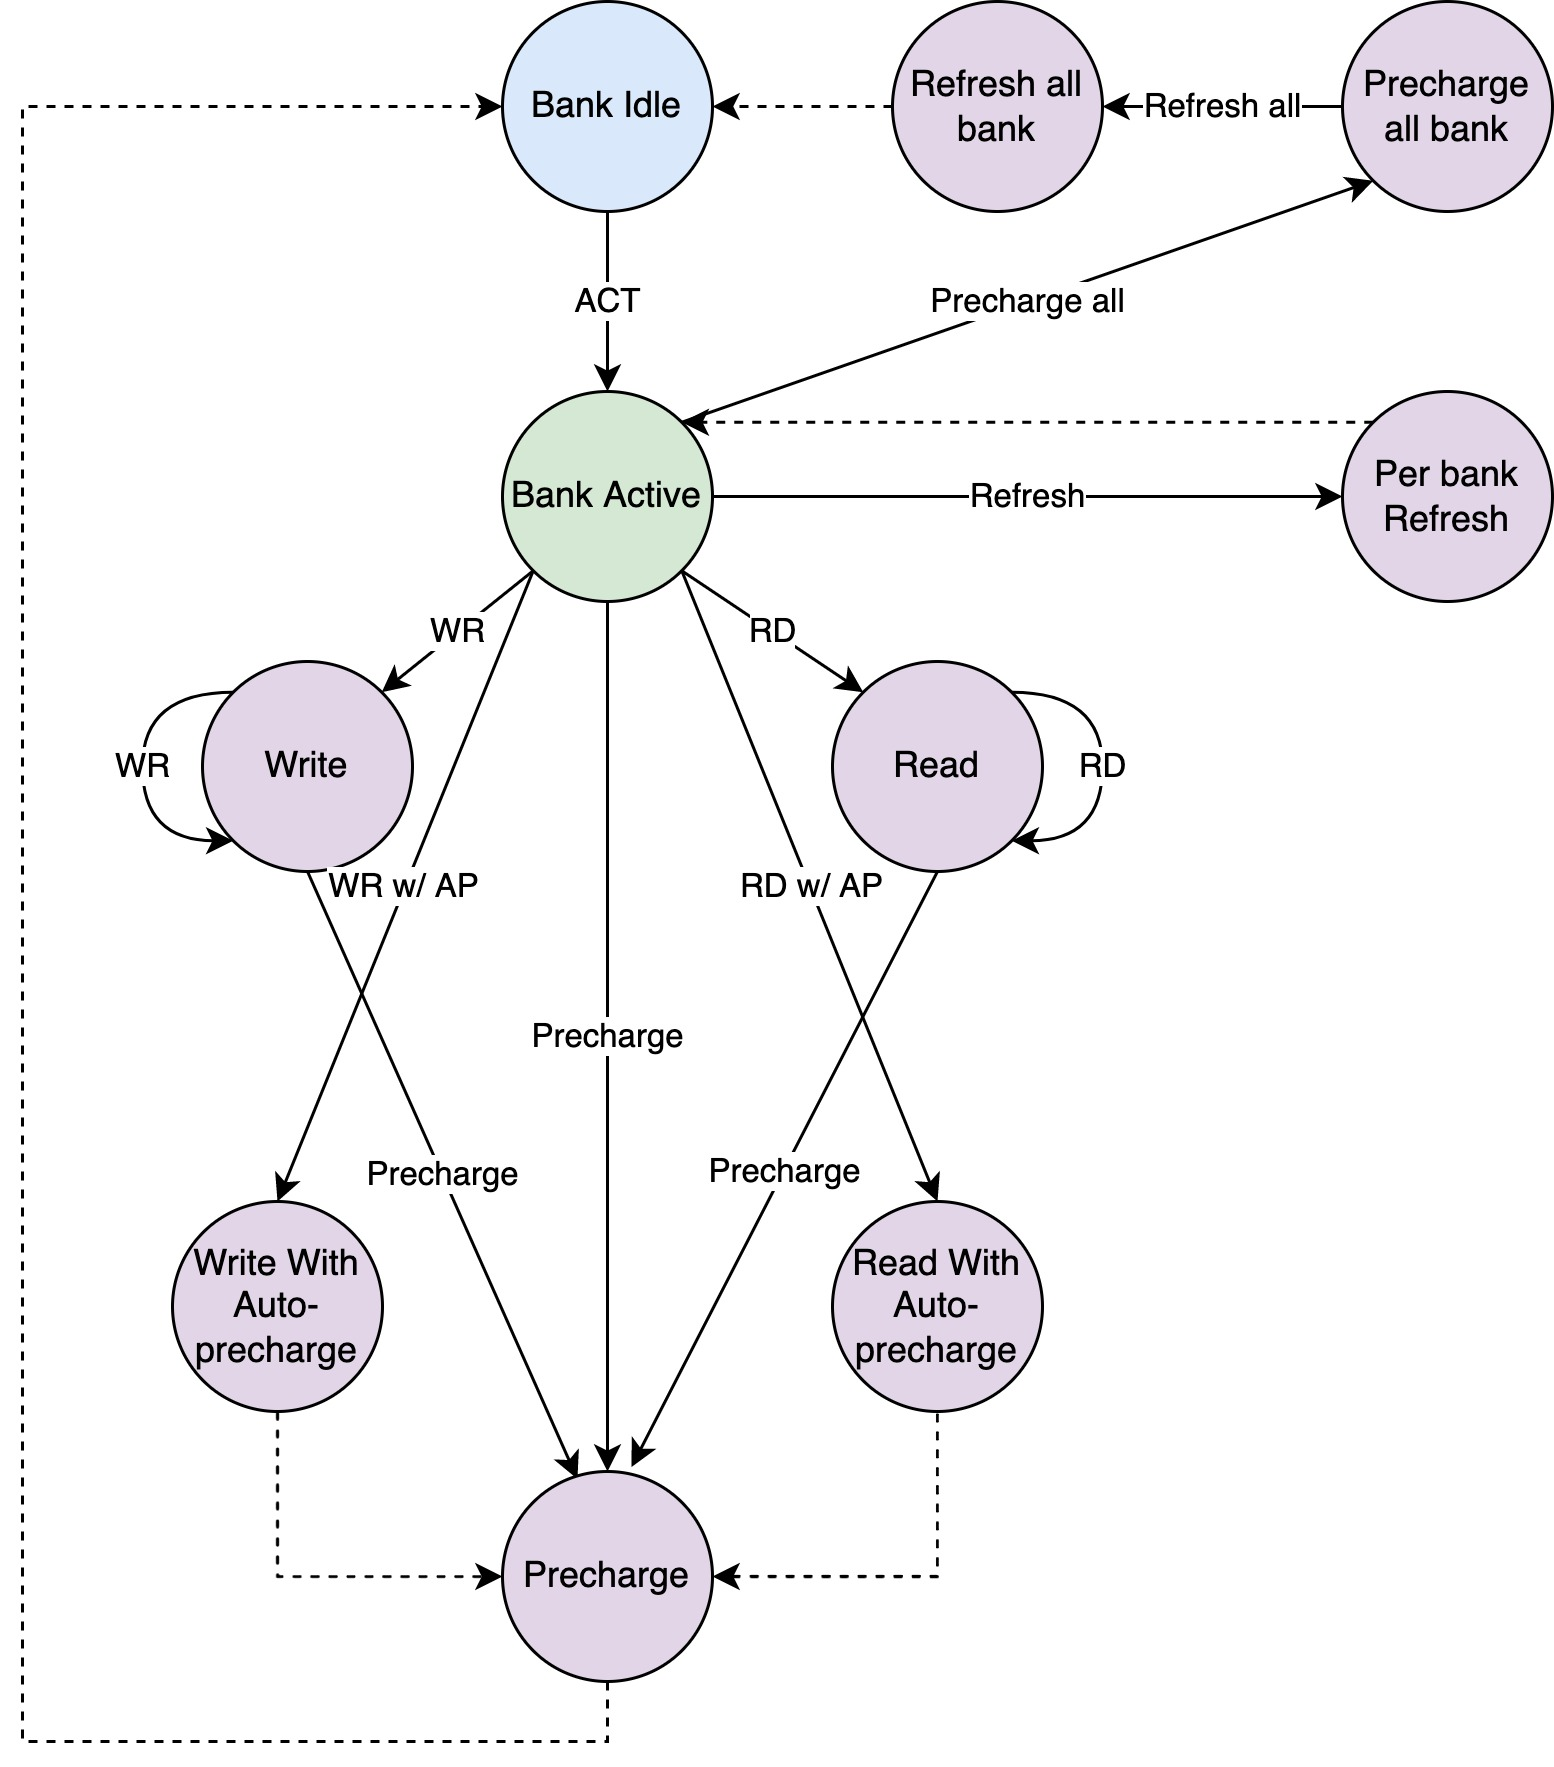
\includegraphics[scale=0.2]{images/fsm.jpg}
    \caption{Per bank state machine.}
    \label{fig:fsm}
\end{figure}

\section{Refresh Controller}
A refresh is needed to maintain the logical value of a bit-cell. This operation is mandatory and due to the leakage of charge from the trench capacitors of the memory cells. A separate controller module is responsible for refreshing the DRAM device. A compatible LPDDR4X memory device can refresh banks individually, or all the banks at the same time. In our design, we have a refresh controller that refreshes all the banks by first issuing a precharge-all command. The precharge-all command must be issued before a refresh since a bank must be in an idle state before a refresh operation. The refresh controller has a counter internally to maintain a timely refresh to the device. TREFI is specified as the average refresh interval with a value of 3.904 microseconds. A counter that counts the number of cycles up to TREFI sends a refresh request to the multiplexer module. Once the request is approved by the multiplexer, the refresh controller takes over the command bus and can start issuing commands. The acknowledgment from the multiplexer is necessary since the multiplexer module ensures that bank machines transition to the idle state. Figure \ref{fig:refall} show an example of the refresh procedure and commands to be sent by the refresh controller. 
\newpage
The first phase for a refresh sequence is to issue a DFI standard command for pre-charge all as below:
\begin{verbatim}
          cmd(0).dfiCs := true.B
          // Precharge-1 Low (default)
          // Precharge-2 Hi
          cmd(2).dfiAddress := "b11_0000".U
          cmd(2).dfiCs := true.B
          // Precharge-2 Low
          cmd(3).dfiAddress := "b00_0000".U
          cmd(3).dfiCs := false.B
\end{verbatim}
\begin{figure}
    \centering
    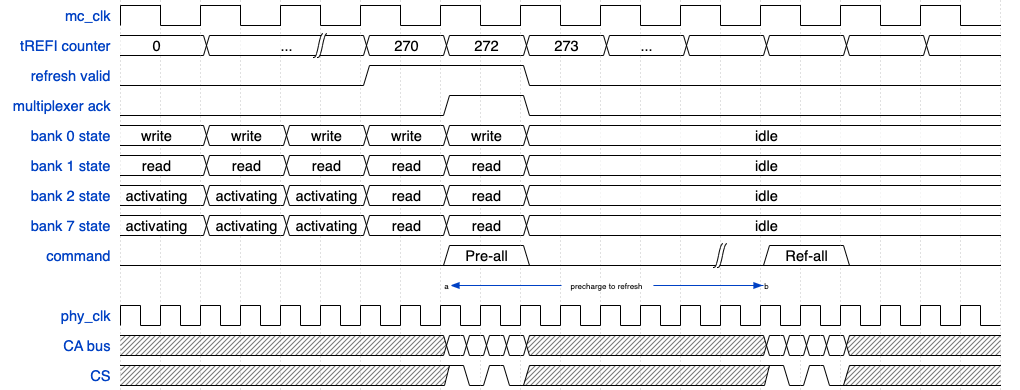
\includegraphics[scale=0.5]{images/refresh-wave.png}
    \caption{Refresh-all sequence.}
    \label{fig:refall}
\end{figure}
The commands are sent over in one cycle of the memory controller; however, each command will be translated into four cycles of DFI clock domain. Each command can be split into four phases of the controller cycle and sent out as a vector of size four. The dfiAddress field in the code snippet above maps to the CA bus which is the command and control bus of the channel. 
\section{Controller Bring-up}
At the time of bring-up, the DDR module in the chip must be configured with the timing parameters and mode register values.

The sample code below shows the timing parameters that need to be configured at the time of bring-up. The configuration is done using the TileLink register node and is done by a core in the system issuing writes to the corresponding address.
\begin{verbatim}
val tphycwl = RegInit(8.U(timeBits.w.W))
val tphycl = RegInit(14.U(timeBits.w.W))
val twr = RegInit(4.U(timeBits.w.W))
node.regmap(
      0x00 -> Seq(RegField(timeBits.w, tphycwl)),
      0x01 -> Seq(RegField(timeBits.w, tphycl)),
      0x02 -> Seq(RegField(timeBits.w, twr)),
      ...)
\end{verbatim}

A bare-metal software can be written to write the timing registers and the device mode registers. 

\section{Scheduling Logic}
The scheduling logic determines which request from each bank can be issued to the device at any cycle. The Bank Machines provide a command that meets the per bank timings to the \verb|CommandChooser| module, where a round-robin arbiter provides an index to pick the next command to be sent. \verb|CommandChooser| module can be optimized to use more sophisticated arbiters to optimize for DQ bandwidth. In addition, a fairer history-based arbiter can be deployed in place of the round-robin arbiter. \footnote{The architecture planning for this unit was done by Ken Ho and me. The implementation of the scheduling logic was done by Ken Ho.
}

\subsection{Open-page Policy}
In an open-page policy mode, the Bank Machines can keep a row open after an activate and a CAS command. Further CAS commands can be issued after a CAS to CAS latency. Open-page policy avoids an activation for the second CAS command. Our design incorporates this idea into the Bank Machine as a configurable parameter. If configured to perform an auto-precharge command, a CAS command automatically performs a precharge and puts the bank in an idle state. However, if not set to use auto-precharge, the look-ahead command buffer in the Bank Machine allows us to check for a row hit. A row hit follows by keeping the row open and issuance of the second CAS command right after. 

A concerning side effect of the open-page policy is the potential starvation of other requests to the same bank in case a row is being accessed regularly. This could be due to an application performing reads and updates to a specific variable or a malicious code accessing one particular variable in a loop to exploit the open-page policy.



\section{Controller Configuration}
Three main case classes are used to configure the LPDDR4 controller based on the design of the SoC and memory system. 

The Geometry class corresponds to the DRAM device configuration, time counter width, depth of the queues in the design, row slice from the address, column slice, and bank slice. This case class can be instantiated in the configuration class of the chip. 

DFI parameters case class corresponds to the DFI-specific parameters used in the design. DFI width, the number of phases per controller clock, and PHY slice widths are all determined in this case class. Similar to the Geometry class, the DFI parameters should be instantiated and modified per design-specific constraints. 

A TileLink parameter case class is also needed to configure the TileLink nodes needed in the design. This case class requires the designer to provide two base addresses. One address for the base of the DRAM. This address should be the base of the memory for the SoC and must be a cachable address range. The other base address is used for the register node and configuration of the timing parameters. The configuration base address can be associated with a control address and should be uncachable. 

The DDR generator has a \verb|CanHaveMasterTLDDRPort| trait. This trait is used as one of the traits that \verb|DigitalChip| inherits. Once added to the \verb|DigitalChip| of Chipyard, the trait instantiates the TileLink module and connects the internal TileLink node for memory to the memory bus of the system. It also connects the internal register node in the TileLink module to the periphery bus of the system. The trait instantiates the DDR top module and connects the interfaces of the top module to the TileLink module. The connection must happen in this way due to TileLink requirements for elaboration and TileLink lazy module system.
\begin{verbatim}
class DigitalTop(implicit p: Parameters) extends ChipyardSystem
    with ddr.CanHaveMasterTLDDRPort

        
class WithDDR(val geom: GeomParams, val dfi: DFIParams, val tl:  TileLinkParams) 
    extends Config((site, here, up) => {
  case DDRKey => Some(DDRParams(geom = geom, dfi = dfi, tl = tl))
})  
\end{verbatim}

A chip configuration with the LPDDR4 memory controller would add \verb|WithDDR| with the intended parameters to instantiate the controller. 

